\chapter{项目管理}


\section{任务计划安排}

\subsection{工作分解}

\begin{enumerate}
    \item Sprint1 工作任务分解表 (10.11-10.31)

          \begin{longtable}{>{\centering\arraybackslash}m{2cm} >{\centering\arraybackslash}m{5cm} >{\centering\arraybackslash}m{5cm} >{\centering\arraybackslash}m{1.5cm}}

              \caption{Sprint1工作任务分解表} \label{tab:training}                                                             \\

              \toprule
              \textbf{层级}        & \textbf{内容（关联迭代）}                  & \textbf{拆解说明}                    & \textbf{负责人} \\
              \midrule
              \endfirsthead

              \multicolumn{4}{c}{{\tablename\ \thetable{} 续表}}                                                          \\
              \toprule
              \textbf{层级}        & \textbf{内容（关联迭代）}                  & \textbf{拆解说明}                    & \textbf{负责人} \\
              \midrule
              \endhead

              \bottomrule
              \endfoot


              1. Product Backlog & US001（用户注册登录）（P0）                  & 大需求：支撑用户端登录入口，纳入 Sprint1         & 贾思韵          \\
              2. Sprint Backlog  & T101（用户注册/登录后端接口）                  & 中需求：Sprint1 的核心任务，前后端拆分          & 戴茗静          \\
              3. 具体任务            & T101-1（用户表设计与注册接口开发）               & 小任务：设计users表、BCrypt加密存储、注册接口     & 戴茗静          \\
              3. 具体任务            & T101-2（登录接口与JWT token签发）           & 小任务：用户名密码验证、JWT生成、24小时会话         & 戴茗静          \\
              3. 具体任务            & T101-3（token验证中间件开发）               & 小任务：Spring Security配置、路由守卫       & 戴茗静          \\
              2. Sprint Backlog  & T102（用户注册/登录前端页面）                  & 中需求：用户登录注册界面                     & 杨晓越          \\
              3. 具体任务            & T102-1（Login.vue登录页面开发）            & 小任务：用户名密码表单、记住我功能                & 杨晓越          \\
              3. 具体任务            & T102-2（Register.vue注册页面开发）         & 小任务：用户信息表单、密码强度校验、确认密码           & 杨晓越          \\
              3. 具体任务            & T102-3（前端路由守卫实现）                   & 小任务：axios拦截器、未登录跳转逻辑             & 杨晓越          \\
              1. Product Backlog & US002（商铺查询）（P0）                    & 大需求：用户发现商铺的核心路径，纳入 Sprint1       & 贾思韵          \\
              2. Sprint Backlog  & T103（商铺查询后端接口）                     & 中需求：提供商铺搜索和分类筛选能力                & 曾意           \\
              3. 具体任务            & T103-1（商铺列表查询接口开发）                 & 小任务：business表设计、分页查询、基础信息返回      & 曾意           \\
              3. 具体任务            & T103-2（商铺分类筛选接口开发）                 & 小任务：按10个品类分类查询、销量排序              & 曾意           \\
              3. 具体任务            & T103-3（商铺关键字搜索接口开发）                & 小任务：商铺名、商品名模糊匹配、按评分销量排序          & 曾意           \\
              3. 具体任务            & T103-4（首页轮播推荐接口开发）                 & 小任务：销量前三商家轮播数据接口                 & 曾意           \\
              2. Sprint Backlog  & T104（商铺查询前端页面）                     & 中需求：用户搜索和浏览商铺的界面                 & 贾思韵          \\
              3. 具体任务            & T104-1（Index.vue首页开发）              & 小任务：分类入口、搜索栏、轮播推荐区域              & 贾思韵          \\
              3. 具体任务            & T104-2（商铺列表筛选组件开发）                 & 小任务：按销量、起送费配送费区间筛选               & 贾思韵          \\
              3. 具体任务            & T104-3（搜索结果页开发）                    & 小任务：搜索结果展示、空结果提示                 & 贾思韵          \\
              1. Product Backlog & US003（商铺详情）（P0）                    & 大需求：用户查看商铺和商品详情，纳入 Sprint1       & 贾思韵          \\
              2. Sprint Backlog  & T105（商铺详情后端接口）                     & 中需求：提供商铺详情和商品列表数据                & 曾意           \\
              3. 具体任务            & T105-1（商铺详情查询接口开发）                 & 小任务：返回商铺图片、名称、配送费、起送价、介绍         & 曾意           \\
              3. 具体任务            & T105-2（商品列表查询接口开发）                 & 小任务：返回已上架商品列表（名称、价格、图片）          & 曾意           \\
              2. Sprint Backlog  & T106（商铺详情前端页面）                     & 中需求：商铺详情展示页面                     & 贾思韵          \\
              3. 具体任务            & T106-1（BusinessInfo.vue商铺详情页开发）    & 小任务：商铺信息展示区域                     & 贾思韵          \\
              3. 具体任务            & T106-2（商品列表组件开发）                   & 小任务：商品卡片展示、价格格式处理                & 贾思韵          \\
              3. 具体任务            & T106-3（页面性能优化）                     & 小任务：确保页面加载<2秒                    & 贾思韵          \\
              1. Product Backlog & US004（收货地址管理）（P0）                  & 大需求：下单流程的必备前提，纳入 Sprint1         & 贾思韵          \\
              2. Sprint Backlog  & T107（收货地址后端接口）                     & 中需求：支持用户地址的增删改查                  & 高灿           \\
              3. 具体任务            & T107-1（地址增删改查接口开发）                 & 小任务：delivery\_address表设计、CRUD接口  & 高灿           \\
              3. 具体任务            & T107-2（手机号双重验证逻辑）                  & 小任务：前后端统一的手机号格式验证（11位，1开头，第二位>2） & 高灿           \\
              2. Sprint Backlog  & T108（收货地址前端页面）                     & 中需求：用户管理地址的界面                    & 杨晓越          \\
              3. 具体任务            & T108-1（UserAddress.vue地址列表页）       & 小任务：展示用户所有地址、默认地址设置              & 杨晓越          \\
              3. 具体任务            & T108-2（AddUserAddress.vue新增地址页）    & 小任务：联系人、手机号、详细地址表单               & 杨晓越          \\
              3. 具体任务            & T108-3（EditUserAddress.vue编辑地址页）   & 小任务：地址信息回显与更新                    & 杨晓越          \\
              1. Product Backlog & US005（购物车支付）（P0）                   & 大需求：平台核心交易闭环，纳入 Sprint1          & 贾思韵          \\
              2. Sprint Backlog  & T109（购物车与订单后端接口）                   & 中需求：支持购物车管理和订单创建                 & 戴茗静          \\
              3. 具体任务            & T109-1（购物车接口开发）                    & 小任务：cart表设计、商品增删改查、实时同步          & 戴茗静          \\
              3. 具体任务            & T109-2（订单创建接口开发）                   & 小任务：orders、orderdetailet表设计、下单逻辑 & 戴茗静          \\
              3. 具体任务            & T109-3（订单总价计算逻辑）                   & 小任务：计算商品总额、配送费、起送费判断             & 戴茗静          \\
              3. 具体任务            & T109-4（支付方式接口开发）                   & 小任务：支付宝、微信支付接口对接（模拟）             & 戴茗静          \\
              2. Sprint Backlog  & T110（购物车与支付前端流程）                   & 中需求：用户完成购物和支付的完整界面               & 贾思韵          \\
              3. 具体任务            & T110-1（商铺详情页购物车组件）                 & 小任务：加购按钮、底部购物车信息展示               & 贾思韵          \\
              3. 具体任务            & T110-2（Cart.vue购物车页面开发）            & 小任务：商品展示、数量修改、总价计算               & 贾思韵          \\
              3. 具体任务            & T110-3（Payment.vue支付页面开发）          & 小任务：地址选择、支付方式选择                  & 贾思韵          \\
              3. 具体任务            & T110-4（SuccessfulPayment.vue支付成功页） & 小任务：支付成功展示、订单号显示                 & 贾思韵          \\
              1. Product Backlog & US007（订单查看）（P1）                    & 大需求：用户查看和管理订单，纳入 Sprint1         & 贾思韵          \\
              2. Sprint Backlog  & T111（订单查询后端接口）                     & 中需求：支持用户查看不同状态订单                 & 戴茗静          \\
              3. 具体任务            & T111-1（订单列表查询接口开发）                 & 小任务：按状态（待支付/待接单/已接单/已完成/已取消）筛选   & 戴茗静          \\
              3. 具体任务            & T111-2（订单详情查询接口开发）                 & 小任务：返回订单详细信息，包含商品详情              & 戴茗静          \\
              3. 具体任务            & T111-3（订单取消接口开发）                   & 小任务：商家接单前用户取消订单逻辑                & 戴茗静          \\
              2. Sprint Backlog  & T112（订单查看前端页面）                     & 中需求：用户查看订单的界面                    & 杨晓越          \\
              3. 具体任务            & T112-1（Order.vue订单列表页开发）           & 小任务：状态筛选、订单卡片展示                  & 杨晓越          \\
              3. 具体任务            & T112-2（订单详情弹窗组件开发）                 & 小任务：展示订单详细信息                     & 杨晓越          \\
              3. 具体任务            & T112-3（订单取消功能实现）                   & 小任务：取消按钮、确认弹窗                    & 杨晓越          \\
              1. Product Backlog & US015（订单推送）（P2）                    & 大需求：订单状态实时推送，提升用户体验              & 贾思韵          \\
              2. Sprint Backlog  & T113（WebSocket推送后端）                & 中需求：实现订单状态实时推送                   & 曾意           \\
              3. 具体任务            & T113-1（WebSocket服务搭建）              & 小任务：建立WebSocket连接                & 曾意           \\
              3. 具体任务            & T113-2（订单状态推送逻辑）                   & 小任务：订单状态变更时实时推送（1秒内）             & 曾意           \\
              3. 具体任务            & T113-3（消息持久化存储）                    & 小任务：notification表设计、消息存储         & 曾意           \\
              2. Sprint Backlog  & T114（消息推送前端）                       & 中需求：接收和显示推送消息                    & 杨晓越          \\
              3. 具体任务            & T114-1（WebSocket客户端集成）             & 小任务：前端WebSocket连接管理              & 杨晓越          \\
              3. 具体任务            & T114-2（消息接收与展示组件）                  & 小任务：消息展示、红点提示                    & 杨晓越          \\
              3. 具体任务            & T114-3（消息点击跳转功能）                   & 小任务：点击消息跳转到订单详情                  & 杨晓越          \\
              2. Sprint Backlog  & T115（Sprint1 联调、测试与部署）             & 中需求：确保Sprint1所有功能集成可用            & 全体成员         \\
              3. 具体任务            & T115-1（前后端接口联调）                    & 小任务：协调前后端，调试所有接口                 & 任晓华          \\
              3. 具体任务            & T115-2（Sprint1 功能集成测试）             & 小任务：按照验收标准测试核心流程                 & 任晓华          \\
              3. 具体任务            & T115-3（生产环境部署与冒烟测试）                & 小任务：将Sprint1成果部署至生产环境            & 曾意           \\
          \end{longtable}

    \item Sprint2 工作任务分解表 (10.31-11.16)

          \begin{longtable}{>{\centering\arraybackslash}m{2cm} >{\centering\arraybackslash}m{5cm} >{\centering\arraybackslash}m{5cm} >{\centering\arraybackslash}m{1.5cm}}

              \caption{Sprint2工作任务分解表} \label{tab:training}                                                                                              \\

              \toprule
              \textbf{层级}        & \textbf{内容（关联迭代）}                 & \textbf{拆解说明}                                                      & \textbf{负责人} \\
              \midrule
              \endfirsthead

              \multicolumn{4}{c}{{\tablename\ \thetable{} 续表}}                                                                                           \\
              \toprule
              \textbf{层级}        & \textbf{内容（关联迭代）}                 & \textbf{拆解说明}                                                      & \textbf{负责人} \\
              \midrule
              \endhead

              \bottomrule
              \endfoot

              1. Product Backlog & US006（成为商家）（P1）                   & 大需求：实现用户提交资料申请成为商家的核心流程，是商家入驻的第一步。                                 & 贾思韵          \\
              2. Sprint Backlog  & T201（商家入驻申请后端接口）                  & 中需求：支持顾客提交商家身份申请，以及申请后的状态管理。                                       & 戴茗静          \\
              3. 具体任务            & T201-1（申请提交与数据模型设计）               & 小任务：设计permission\_application表，开发/api/permission/apply提交接口，保存申请信息。 & 戴茗静          \\
              3. 具体任务            & T201-2（申请列表与详情查询接口）               & 小任务：开发/api/permission/my-application接口，供用户查看自己的申请状态和详情。            & 戴茗静          \\
              3. 具体任务            & T201-3（申请信息校验逻辑）                  & 小任务：验证申请信息的完整性（如身份证、营业执照等必要字段）。                                    & 戴茗静          \\
              2. Sprint Backlog  & T202（商家入驻申请前端页面）                  & 中需求：用户申请成为商家的操作界面。                                                 & 杨晓越          \\
              3. 具体任务            & T202-1（ApplyMerchant.vue页面开发）     & 小任务：创建表单页面，包含个人信息、资质证明上传等输入项。                                      & 杨晓越          \\
              3. 具体任务            & T202-2（文件上传组件集成）                  & 小任务：集成OSS上传组件，实现资质文件的上传与预览。                                        & 杨晓越          \\
              3. 具体任务            & T202-3（申请提交与状态提示）                 & 小任务：实现表单提交逻辑，提交后清晰展示“审核中”状态。                                       & 杨晓越          \\
              1. Product Backlog & US008（商品管理）（P1）                   & 大需求：商家对店铺商品进行全生命周期管理的核心能力。                                         & 贾思韵          \\
              2. Sprint Backlog  & T203（商品管理后端接口）                    & 中需求：提供商品的增、删、改、查、上下架全套接口。                                          & 高灿           \\
              3. 具体任务            & T203-1（商品CRUD接口开发）                & 小任务：开发/api/foods相关接口，实现商品创建、查询、修改、删除。                              & 高灿           \\
              3. 具体任务            & T203-2（商品上架/下架状态接口）               & 小任务：开发/api/foods/status接口，控制商品的可售状态。                               & 高灿           \\
              3. 具体任务            & T203-3（商品图片上传与管理）                 & 小任务：开发商品图片上传接口，并关联至商品信息。                                           & 高灿           \\
              3. 具体任务            & T203-4（权限校验中间件）                   & 小任务：为所有商品接口添加校验，确保仅商家本人或管理员可操作。                                    & 高灿           \\
              2. Sprint Backlog  & T204（商品管理前端页面）                    & 中需求：商家管理店铺商品的操作界面。                                                 & 贾思韵          \\
              3. 具体任务            & T204-1（MerchantFood.vue商品列表页开发）   & 小任务：展示本店商品列表，支持按状态筛选，包含操作按钮。                                       & 贾思韵          \\
              3. 具体任务            & T204-2（商品新增/编辑弹窗组件）               & 小任务：开发表单弹窗，用于添加新商品或编辑现有商品信息。                                       & 贾思韵          \\
              3. 具体任务            & T204-3（商品操作交互与反馈）                 & 小任务：实现上架、下架、删除等操作的按钮逻辑和结果提示。                                       & 贾思韵          \\
              1. Product Backlog & US011（收藏点赞）（P0）                   & 大需求：增强用户粘性与商铺评价体系的互动功能。                                            & 贾思韵          \\
              2. Sprint Backlog  & T205（用户互动后端接口）                    & 中需求：处理收藏、点赞的点击行为，并维护相关数据。                                          & 曾意           \\
              3. 具体任务            & T205-1（互动接口开发）                    & 小任务：开发/api/merchant/interaction统一接口，处理收藏/点赞的添加与取消。                 & 曾意           \\
              3. 具体任务            & T205-2（用户收藏列表接口）                  & 小任务：开发/api/user/favorites接口，获取用户收藏的商铺列表。                           & 曾意           \\
              3. 具体任务            & T205-3（商铺互动数据聚合查询）                & 小任务：开发接口，快速查询商铺的实时点赞数、收藏数。                                         & 曾意           \\
              3. 具体任务            & T205-4（互动状态同步机制）                  & 小任务：确保商家端统计数据与用户前端展示数据在5秒内同步。                                      & 曾意           \\
              2. Sprint Backlog  & T206（用户互动前端功能）                    & 中需求：在用户端实现收藏、点赞的交互界面。                                              & 杨晓越          \\
              3. 具体任务            & T206-1（BusinessInfo.vue互动按钮组件）    & 小任务：在商铺详情页集成可点击的收藏和点赞按钮，实现状态切换与即时反馈。                               & 杨晓越          \\
              3. 具体任务            & T206-2（Favorites.vue我的收藏页面）       & 小任务：开发独立页面，展示用户收藏的所有商铺，并可跳转至详情页。                                   & 杨晓越          \\
              3. 具体任务            & T206-3（互动状态初始化与持久化）               & 小任务：用户登录后，初始化各商铺的收藏/点赞状态，并确保页面间状态一致。                               & 杨晓越          \\
              1. Product Backlog & US017（商家经营人气统计）（P2）               & 大需求：为商家提供商铺人气数据概览，帮助商家了解店铺受欢迎程度。                                   & 贾思韵          \\
              2. Sprint Backlog  & T207（商家人气统计后端接口）                  & 中需求：提供商家名下所有商铺的点赞数、收藏数、综合评分统计。                                     & 曾意           \\
              3. 具体任务            & T207-1（商铺互动数据聚合接口）                & 小任务：开发/api/merchant/interaction/stats接口，聚合计算每个商铺的点赞数和收藏数。          & 曾意           \\
              3. 具体任务            & T207-2（综合评分计算逻辑）                  & 小任务：实现点赞与收藏加权归一化算法，计算综合评分（如：评分 = 点赞数×0.7 + 收藏数×0.3）。               & 曾意           \\
              3. 具体任务            & T207-3（多商铺数据汇总）                   & 小任务：支持商家查看名下所有商铺的人气数据汇总（总点赞数、总收藏数、平均评分）。                           & 曾意           \\
              3. 具体任务            & T207-4（数据缓存与性能优化）                 & 小任务：对人统计数据进行缓存，确保查询响应时间＜1秒。                                        & 曾意           \\
              2. Sprint Backlog  & T208（商家人气统计前端展示）                  & 中需求：在商家后台清晰展示商铺人气数据。                                               & 杨晓越          \\
              3. 具体任务            & T208-1（MerchantStats.vue人气统计页面开发） & 小任务：开发专门的人气统计页面，按商铺展示点赞数、收藏数、综合评分。                                 & 杨晓越          \\
              3. 具体任务            & T208-2（数据排序与筛选功能）                 & 小任务：支持按评分进行排序，方便用户对比各商铺人气。                                         & 杨晓越          \\
              2. Sprint Backlog  & T209（Sprint2 集成、测试与部署）            & 中需求：确保本迭代所有功能完整、可用、可交付。                                            & 全体成员         \\
              3. 具体任务            & T209-1（商家端完整流程联调）                 & 小任务：从申请到商品管理、接单（如果涉及）的全流程端到端测试。                                    & 任晓华          \\
              3. 具体任务            & T209-2（用户互动功能测试）                  & 小任务：全面测试收藏、点赞功能的正确性、实时性和状态一致性。                                     & 任晓华          \\
              3. 具体任务            & T209-3（Bug修复与代码审查）                & 小任务：修复联调中发现的问题，完成关键代码的合并前审查。                                       & 戴茗静 / 曾意     \\
              3. 具体任务            & T209-4（Sprint2 预生产环境部署与冒烟测试）      & 小任务：将Sprint2成果部署至测试环境，并进行基本功能验证。                                   & 曾意           \\
          \end{longtable}

    \item Sprint3 工作任务分解表（11.17-12.7）

          \begin{longtable}{>{\centering\arraybackslash}m{2cm} >{\centering\arraybackslash}m{5cm} >{\centering\arraybackslash}m{5cm} >{\centering\arraybackslash}m{1.5cm}}

              \caption{Sprint3工作任务分解表} \label{tab:training}                                                                         \\

              \toprule
              \textbf{层级}        & \textbf{内容（关联迭代）}                   & \textbf{拆解说明}                               & \textbf{负责人} \\
              \midrule
              \endfirsthead

              \multicolumn{4}{c}{{\tablename\ \thetable{} 续表}}                                                                      \\
              \toprule
              \textbf{层级}        & \textbf{内容（关联迭代）}                   & \textbf{拆解说明}                               & \textbf{负责人} \\
              \midrule
              \endhead

              \bottomrule
              \endfoot

              1. Product Backlog & US009（商家申请审核）（P1）                   & 大需求：管理员审批商家入驻申请，完善平台治理，纳入 Sprint3           & 贾思韵          \\
              2. Sprint Backlog  & T301（商家申请审核后端接口）                    & 中需求：提供审核列表查询、详情查看、审核操作接口                    & 高灿           \\
              3. 具体任务            & T301-1（商家申请列表查询接口开发）                & 小任务：查询待审核 / 已审核商家申请列表，支持分页                  & 高灿           \\
              3. 具体任务            & T301-2（商家申请详情接口开发）                  & 小任务：返回商家申请完整信息（用户名、手机号、申请时间等）               & 高灿           \\
              3. 具体任务            & T301-3（商家申请审核操作接口开发）                & 小任务：支持 “批准 / 拒绝” 操作，更新权限与状态                 & 高灿           \\
              2. Sprint Backlog  & T302（商家申请审核前端页面）                    & 中需求：管理员审核商家申请的操作界面                          & 贾思韵          \\
              3. 具体任务            & T302-1（AdminAudit.vue 审核列表页开发）      & 小任务：展示申请列表，支持筛选、查看详情                        & 贾思韵          \\
              3. 具体任务            & T302-2（审核操作组件开发）                    & 小任务：实现批准 / 拒绝按钮、二次确认弹窗、结果提示                 & 贾思韵          \\
              1. Product Backlog & US010（商铺申请审核）（P1）                   & 大需求：管理员审批新增商铺申请，纳入 Sprint3                  & 贾思韵          \\
              2. Sprint Backlog  & T303（商铺申请审核后端接口）                    & 中需求：提供商铺申请查询、审核接口                           & 高灿           \\
              3. 具体任务            & T303-1（商铺申请列表查询接口开发）                & 小任务：查询待审核商铺申请，展示核心信息（商铺名、类型、申请时间）           & 高灿           \\
              3. 具体任务            & T303-2（商铺申请详情接口开发）                  & 小任务：返回商铺完整申请信息（地址、介绍、图片等）                   & 高灿           \\
              3. 具体任务            & T303-3（商铺申请审核操作接口开发）                & 小任务：审核通过 / 拒绝，更新商铺状态（待审核→已上线 / 未通过）         & 高灿           \\
              2. Sprint Backlog  & T304（商铺申请审核前端页面）                    & 中需求：管理员审核商铺申请的操作界面                          & 贾思韵          \\
              3. 具体任务            & T304-1（AdminShopAudit.vue 审核列表页开发）  & 小任务：展示商铺申请列表，支持筛选、查看详情                      & 贾思韵          \\
              3. 具体任务            & T304-2（商铺详情预览组件开发）                  & 小任务：预览商铺申请信息，提供审核操作入口                       & 贾思韵          \\
              1. Product Backlog & US012（用户管理）（P1）                     & 大需求：管理员管理用户账号（启用 / 禁用 / 搜索），纳入 Sprint3      & 贾思韵          \\
              2. Sprint Backlog  & T305（用户管理后端接口）                      & 中需求：提供用户搜索、状态管理接口                           & 戴茗静          \\
              3. 具体任务            & T305-1（用户模糊搜索接口开发）                  & 小任务：支持按用户名 / 手机号 / 邮箱搜索，响应时间 < 1 秒          & 戴茗静          \\
              3. 具体任务            & T305-2（用户状态筛选接口开发）                  & 小任务：按 “已启用 / 已禁用” 筛选用户列表                    & 戴茗静          \\
              3. 具体任务            & T305-3（用户启用 / 禁用接口开发）               & 小任务：修改用户 activated 字段，支持二次确认                & 戴茗静          \\
              2. Sprint Backlog  & T306（用户管理前端页面）                      & 中需求：管理员管理用户的操作界面                            & 杨晓越          \\
              3. 具体任务            & T306-1（UserManagement.vue 用户列表页开发）  & 小任务：展示用户基本信息、注册时间、状态                        & 杨晓越          \\
              3. 具体任务            & T306-2（用户搜索与筛选组件开发）                 & 小任务：实现搜索框、状态筛选下拉框                           & 杨晓越          \\
              3. 具体任务            & T306-3（启用 / 禁用操作组件开发）               & 小任务：按钮触发二次确认，操作成功即时更新状态                     & 杨晓越          \\
              1. Product Backlog & US013（商铺管理）（P1）                     & 大需求：管理员集中管理商家集团与商铺，纳入 Sprint3               & 贾思韵          \\
              2. Sprint Backlog  & T307（商铺管理后端接口）                      & 中需求：提供商铺增删改查接口                              & 戴茗静          \\
              3. 具体任务            & T307-1（商家集团与商铺关联查询接口开发）             & 小任务：查询所有商家集团及下属商铺，加载时间 < 1 秒                & 戴茗静          \\
              3. 具体任务            & T307-2（商铺新增接口开发）                    & 小任务：管理员直接新增商铺，无需审核                          & 戴茗静          \\
              3. 具体任务            & T307-3（商铺编辑接口开发）                    & 小任务：修改商铺名称、地址、起送费等字段                        & 戴茗静          \\
              3. 具体任务            & T307-4（商铺删除接口开发）                    & 小任务：逻辑删除商铺，支持二次确认                           & 戴茗静          \\
              2. Sprint Backlog  & T308（商铺管理前端页面）                      & 中需求：管理员管理商铺的操作界面                            & 杨晓越          \\
              3. 具体任务            & T308-1（AdminBusiness.vue 商家集团列表页开发） & 小任务：展示商家集团列表，支持展开下属商铺                       & 杨晓越          \\
              3. 具体任务            & T308-2（商铺管理组件开发）                    & 小任务：实现商铺新增 / 编辑 / 删除操作按钮与表单                 & 杨晓越          \\
              1. Product Backlog & US014（AI 客服）（P2）                    & 大需求：顾客通过 AI 智能助手咨询，纳入 Sprint3               & 贾思韵          \\
              2. Sprint Backlog  & T309（AI 客服后端接口）                     & 中需求：提供 AI 问答、对话历史接口                         & 曾意           \\
              3. 具体任务            & T309-1（ai\_chat\_history 表设计）       & 小任务：设计对话存储表（用户 ID、会话 ID、消息内容等）              & 曾意           \\
              3. 具体任务            & T309-2（AI 问答接口开发）                   & 小任务：集成 DeepSeek API，响应时间 < 3 秒              & 曾意           \\
              3. 具体任务            & T309-3（对话历史查询接口开发）                  & 小任务：查询用户历史对话记录                              & 曾意           \\
              2. Sprint Backlog  & T310（AI 客服前端页面）                     & 中需求：AI 智能助手交互界面                             & 贾思韵          \\
              3. 具体任务            & T310-1（AIChat.vue 聊天页面开发）           & 小任务：悬浮入口、聊天窗口、消息展示区域                        & 贾思韵          \\
              3. 具体任务            & T310-2（消息发送与接收组件开发）                 & 小任务：输入框、发送按钮、AI 响应展示                        & 贾思韵          \\
              3. 具体任务            & T310-3（对话历史展示组件开发）                  & 小任务：查看历史对话记录                                & 贾思韵          \\
              1. Product Backlog & US016（审核结果通知）（P2）                   & 大需求：实时推送审核结果给申请人，纳入 Sprint3                 & 贾思韵          \\
              2. Sprint Backlog  & T311（审核通知后端接口）                      & 中需求：WebSocket 推送审核结果                        & 曾意           \\
              3. 具体任务            & T311-1（审核结果通知推送逻辑开发）                & 小任务：审核操作后 1 秒内推送通知                          & 曾意           \\
              3. 具体任务            & T311-2（通知持久化接口开发）                   & 小任务：将通知存入 notification 表                    & 曾意           \\
              2. Sprint Backlog  & T312（审核通知前端页面）                      & 中需求：消息通知展示与交互                               & 杨晓越          \\
              3. 具体任务            & T312-1（消息通知中心优化）                    & 小任务：展示审核结果通知，红点提示未读                         & 杨晓越          \\
              3. 具体任务            & T312-2（快捷入口组件开发）                    & 小任务：审核通过时显示 “立即去开店 / 切换身份” 入口               & 杨晓越          \\
              1. Product Backlog & US018（平台统计）（P2）                     & 大需求：管理员查看平台经营指标，纳入 Sprint3                  & 贾思韵          \\
              2. Sprint Backlog  & T313（平台统计后端接口）                      & 中需求：提供用户数、店铺数、营业额统计接口                       & 戴茗静          \\
              3. 具体任务            & T313-1（总用户数统计接口开发）                  & 小任务：查询 users 表有效用户总数                        & 戴茗静          \\
              3. 具体任务            & T313-2（总店铺数统计接口开发）                  & 小任务：查询 business 表已上线店铺总数                    & 戴茗静          \\
              3. 具体任务            & T313-3（总营业额统计接口开发）                  & 小任务：统计 orders 表订单总价总和                       & 戴茗静          \\
              2. Sprint Backlog  & T314（平台统计前端页面）                      & 中需求：数据看板展示页面                                & 贾思韵          \\
              3. 具体任务            & T314-1（AdminDashboard.vue 数据看板开发）   & 小任务：展示三合一数据卡片（用户数、店铺数、营业额）                  & 贾思韵          \\
              1. Product Backlog & US019（系统安全）（P1）                     & 大需求：保障用户数据安全与接口稳定，纳入 Sprint3                & 贾思韵          \\
              2. Sprint Backlog  & T315（系统安全后端优化）                      & 中需求：接口鉴权、安全防护优化                             & 高灿 / 戴茗静     \\
              3. 具体任务            & T315-1（接口鉴权增强开发）                    & 小任务：所有接口 JWT 校验，无 token 返回 401              & 高灿           \\
              3. 具体任务            & T315-2（SQL 注入防护开发）                  & 小任务：参数绑定、输入过滤，防护通过率 100\%                   & 戴茗静          \\
              3. 具体任务            & T315-3（XSS 防护开发）                    & 小任务：前端输入过滤、后端输出编码                           & 戴茗静          \\
              2. Sprint Backlog  & T316（系统安全前端优化）                      & 中需求：请求拦截、异常处理优化                             & 杨晓越          \\
              3. 具体任务            & T316-1（axios 拦截器优化）                 & 小任务：请求携带 token、网络错误重试 3 次                   & 杨晓越          \\
              3. 具体任务            & T316-2（全局异常提示组件开发）                  & 小任务：统一展示接口异常信息                              & 杨晓越          \\
              2. Sprint Backlog  & T317（Sprint3 联调、测试与部署）              & 中需求：确保所有功能集成可用、达标上线                         & 全体成员         \\
              3. 具体任务            & T317-1（管理员端全模块联调）                   & 小任务：协调前后端，调试所有管理端接口                         & 任晓华          \\
              3. 具体任务            & T317-2（专项测试：AI 客服、安全、统计）            & 小任务：按验收标准测试专项功能                             & 任晓华          \\
              3. 具体任务            & T317-3（性能压测与安全扫描）                   & 小任务：执行系统压力测试、安全漏洞扫描                         & 曾意           \\
              3. 具体任务            & T317-4（生产环境预部署与冒烟测试）                & 小任务：部署预生产环境，验证核心功能                          & 曾意           \\
              1. Product Backlog & US017（商家经营人气统计）（P2）                 & 补充实时同步优化，纳入 Sprint3                         & 贾思韵          \\
              2. Sprint Backlog  & T318（US017 实时同步优化）                  & 中需求：实现统计数据误差≤2 秒                            & 曾意 / 杨晓越     \\
              3. 具体任务            & T318-1（缓存刷新机制开发）                    & 小任务：设计 1 秒缓存刷新逻辑，关联 merchant\_interaction 表 & 曾意           \\
              3. 具体任务            & T318-2（前端实时刷新优化）                    & 小任务：WebSocket 监听缓存变更 + 定时轮询兜底               & 杨晓越          \\
              3. 具体任务            & T318-3（性能测试与调优）                     & 小任务：模拟并发场景验证同步延迟                            & 任晓华          \\
          \end{longtable}

\end{enumerate}

\subsection{任务估算}

\begin{levellist}
    \item \textbf{估算方法与标准}
    \begin{levellist}
        \item 估算方法：采用规划扑克法，前后端全体核心成员共同参与，基于斐波那契数列（1/2/3/5/8）估算用户故事点，1 个故事点对应 4 个有效开发工时（不含沟通、联调等非编码时间）。
        \item 估算维度：综合任务复杂度（技术难度、逻辑复杂度）、工作量（代码量、测试覆盖度）、依赖关系（跨模块 / 外部依赖）三大维度，确保估算客观可追溯。
        \item 校准机制：每个迭代结束后，对比 “预估工时” 与 “实际工时”，更新估算校准系数，后续迭代估算时动态调整，符合 CMM3 级 “估算可追溯、可优化” 要求。
    \end{levellist}


    \item \textbf{估算结果（按迭代）}

    \begin{longtable}{>{\centering\arraybackslash}m{1.5cm} >{\centering\arraybackslash}m{4cm} >{\centering\arraybackslash}m{1.2cm} >{\centering\arraybackslash}m{2.3cm} >{\centering\arraybackslash}m{3.2cm}}

        \caption{任务估算结果} \label{tab:training}                                                                                                                      \\

        \toprule
        \textbf{迭代}          & \textbf{包含用户故事}                                 & \textbf{总故事点} & \textbf{总预估工时（故事点 ×4）} & \textbf{实际工时（Sprint 详情记录）}               \\
        \midrule
        \endfirsthead

        \multicolumn{8}{c}{{\tablename\ \thetable{} 续表}}                                                                                                           \\
        \toprule
        \textbf{迭代}          & \textbf{包含用户故事}                                 & \textbf{总故事点} & \textbf{总预估工时（故事点 ×4）} & \textbf{实际工时（Sprint 详情记录）}               \\
        \midrule
        \endhead

        \bottomrule
        \endfoot

        Sprint1（10.11-10.30） & US001、US002、US003、US004、US005、US007、US015       & 39            & 156 小时                 & 128 小时（前端 61 小时 + 后端 67 小时）              \\
        Sprint2（10.31-11.16） & US006、US008、US011、US017                         & 14            & 56 小时                  & 64 小时（前端 24 小时 + 后端 30 小时 + 测试与部署 10 小时） \\
        Sprint3（11.17-12.7）  & US009、US010、US012、US013、US014、US016、US018、US019 & 24            & 96 小时                  & 98 小时（前端 31 小时 + 后端 45 小时 + 测试与部署 22 小时） \\
    \end{longtable}



    \begin{longtable}{>{\centering\arraybackslash}m{2cm} >{\centering\arraybackslash}m{2cm} >{\centering\arraybackslash}m{2cm} >{\centering\arraybackslash}m{7.5cm}}

        \caption{任务估算结果（偏差）} \label{tab:training}                                                                          \\

        \toprule
        \textbf{迭代}          & \textbf{偏差量} & \textbf{偏差率} & \textbf{偏差原因分析}                                               \\
        \midrule
        \endfirsthead

        \multicolumn{4}{c}{{\tablename\ \thetable{} 续表}}                                                                   \\
        \toprule
        \textbf{迭代}          & \textbf{偏差量} & \textbf{偏差率} & \textbf{偏差原因分析}                                               \\
        \midrule
        \endhead

        \bottomrule
        \endfoot


        Sprint1（10.11-10.30） & -28 小时       & -17.9\%      & 1. 预估时未充分考虑团队成员技术熟练度，实际开发效率高于预期； \newline
        2. 数据库设计提前完成，为接口开发节省时间； \newline
        3. 核心功能模块拆分合理，并行开发减少等待时间； \newline
        4. 部分非核心测试工作（如兼容性测试）延迟至 Sprint2，减少当期工时占用。                                                                          \\
        Sprint2（10.31-11.16） & +8 小时        & +14.2\%      & 1. US008 商品管理接口权限校验逻辑复杂度超预期，多耗时 3 小时； \newline
        2. 预生产环境部署时服务器配置调试耗时 5 小时，超出初期预估。                                                                                  \\
        Sprint3（11.17-12.7）  & +2 小时        & +2.1\%       & 1. AI 客服接口集成 DeepSeek 时，遇到定义接口与文档不一致情况，实际开发耗时多 1 小时； \newline
        2. 性能压测没有提前规划，环境搭建效率降低，多耗时 1 小时。                                                                                   \\
    \end{longtable}


    \item \textbf{各迭代估算结果与偏差分析}
    \begin{levellist}
        \item \textbf{Sprint1 回顾}
        Sprint1作为项目开端，估算时采用了较为保守的策略。实际执行中，得益于团队成员对技术栈熟悉、核心模块拆分合理以及部分非核心工作，如深度兼容性测试后置，整体开发效率高于预期，形成了显著的\textbf{正向偏差}。这表明初始的工时转换系数（4小时/故事点）对本团队而言可能偏高。

        \item \textbf{Sprint2 回顾}
        在Sprint1高效完成的乐观情况下，团队维持了原有估算策略。但本迭代遇到了两个典型问题：
        \begin{levellist}
            \item \textbf{技术复杂度低估：} US008（商品管理）的精细化权限校验逻辑比预想复杂，增加了后端开发时间。
            \item \textbf{环境与部署成本：} 首次进行集成部署时，服务器环境配置和调试消耗了未在故事点中体现的额外时间。
            这导致了负向偏差（超支工时），提醒团队需要在估算中为“技术未知数”和“运维开销”留出缓冲。
        \end{levellist}

        \item \textbf{Sprint3 回顾} \\
        在吸收了前两个迭代的经验后，本迭代的估算非常接近实际。微小的超支主要来自：
        \begin{levellist}
            \item \textbf{外部依赖风险：} 集成DeepSeek API时遇到接口与文档的细微不一致，增加了联调时间。
            \item \textbf{专项测试准备：} 性能压测环境搭建的效率略低于预期。
        \end{levellist}
        仅2.1\% 的偏差率表明，团队的估算能力、任务拆解水平和风险预判已经趋于成熟和稳定。

        \item \textbf{整体趋势与校准总结}
        \begin{itemize}
            \item 估算偏差从 -17.9\% → +14.3\ → +2.1\%，波动幅度迅速收窄，并稳定在非常低的水平。这清晰展示了团队从“保守探索”到“遭遇技术债”，再到“精准预测”的成熟过程。
            \item 整体校准系数：290 / 308 ≈ 0.94
            \item 对于本项目团队和技术栈，每个故事点约对应 3.76 工时（即 4小时/点 × 0.94）。核心原因在于：
                  \begin{levellist}
                      \item 团队成长：对业务和技术栈的熟悉度持续提升，开发效率稳步提高。
                      \item 资产复用：前端组件、后端通用模块的复用率高于初期预期，减少了重复开发。
                      \item 估算细化：任务拆解更细致，对“非功能需求”（如部署、压测）的工时安排更为明确。
                  \end{levellist}
        \end{itemize}
    \end{levellist}


\end{levellist}


\subsection{甘特图}

\begin{figure}[H]
    \centering
    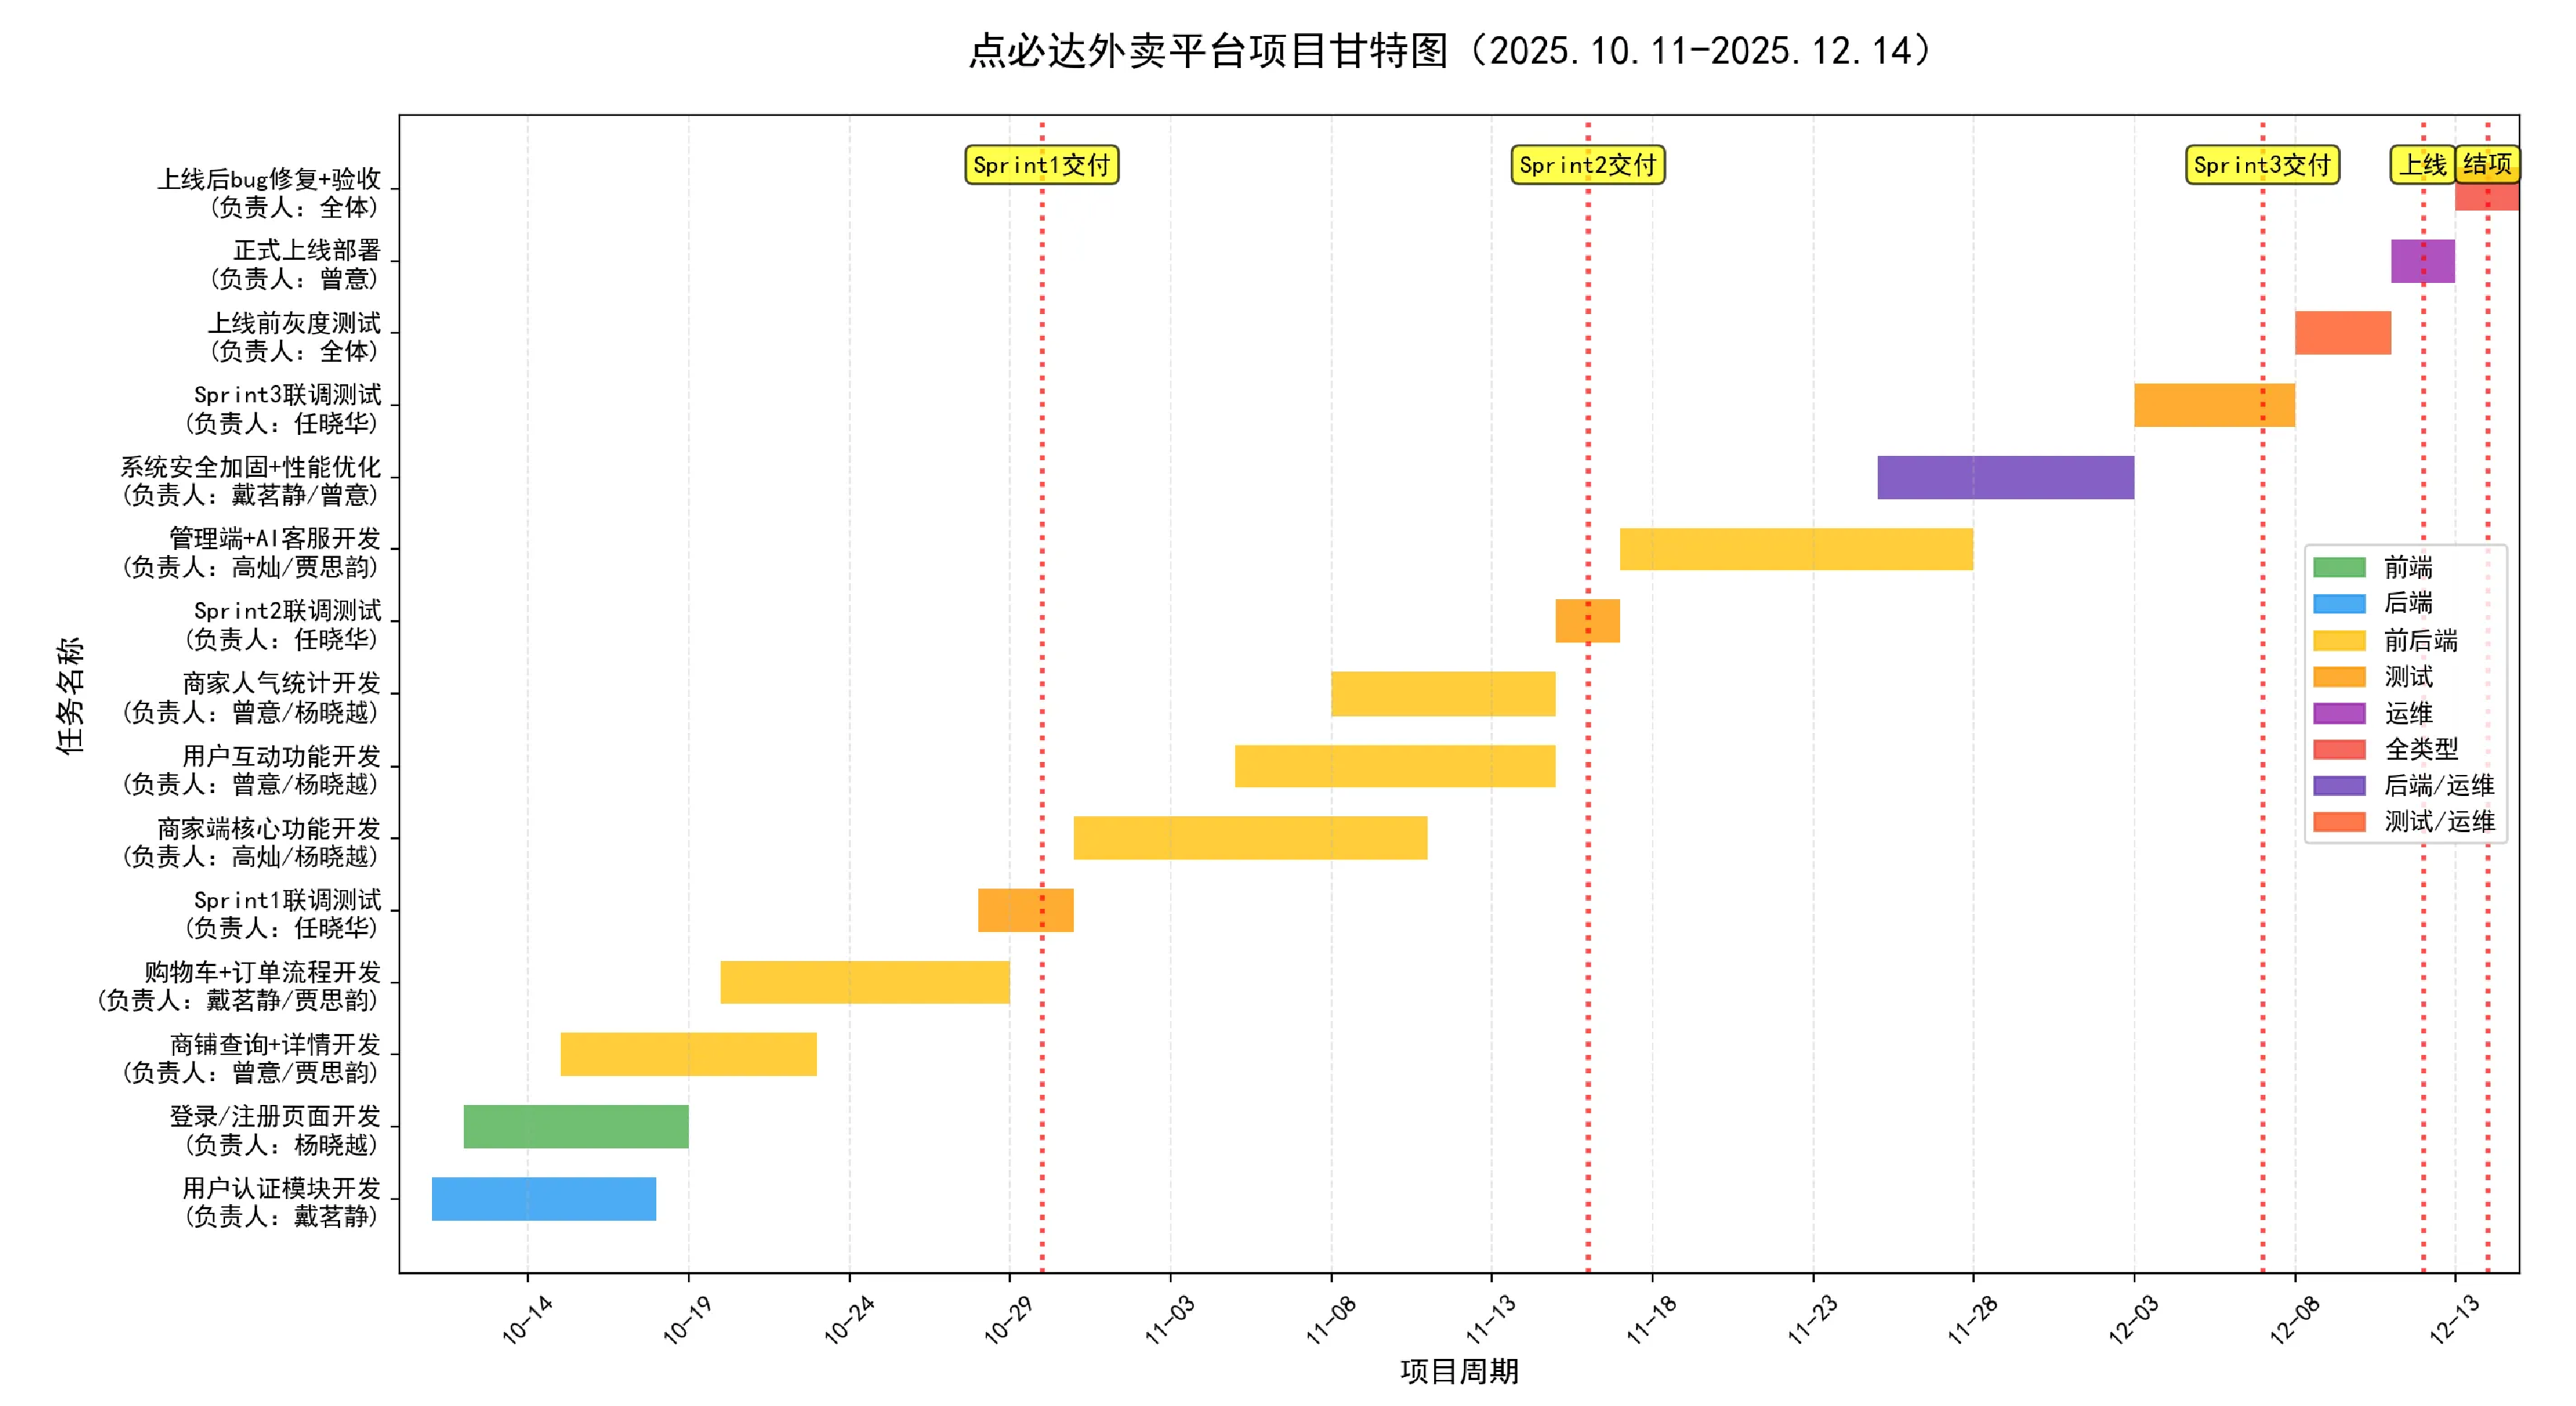
\includegraphics[width=1\textwidth]{figures/in/image4}
    \caption{项目甘特图}
\end{figure}

\subsection{项目整体燃尽图}
\begin{enumerate}
    \item \textbf{燃尽图基础信息}
          \begin{itemize}
              \item 项目总周期：2025 年 10 月 11 日 - 2025 年 12 月 14 日（含 3 个 Sprint 迭代 + 上线准备，共 64 个工作日）
              \item 跟踪对象：项目所有 Product Backlog 任务（总故事点 77 点，含 P0 核心 31 点、P1 重要 32 点、P2 优化 14 点）
              \item 数据来源：各 Sprint 燃尽图的 “实际剩余故事点” 汇总，结合每日站会进度同步数据
              \item 核心目标：12 月 14 日前完成所有 P0/P1 需求及关键 P2 功能，交付可上线的完整版本
          \end{itemize}

    \item[]

    \item \textbf{整体燃尽图}
          \begin{figure}[H]
              \centering
              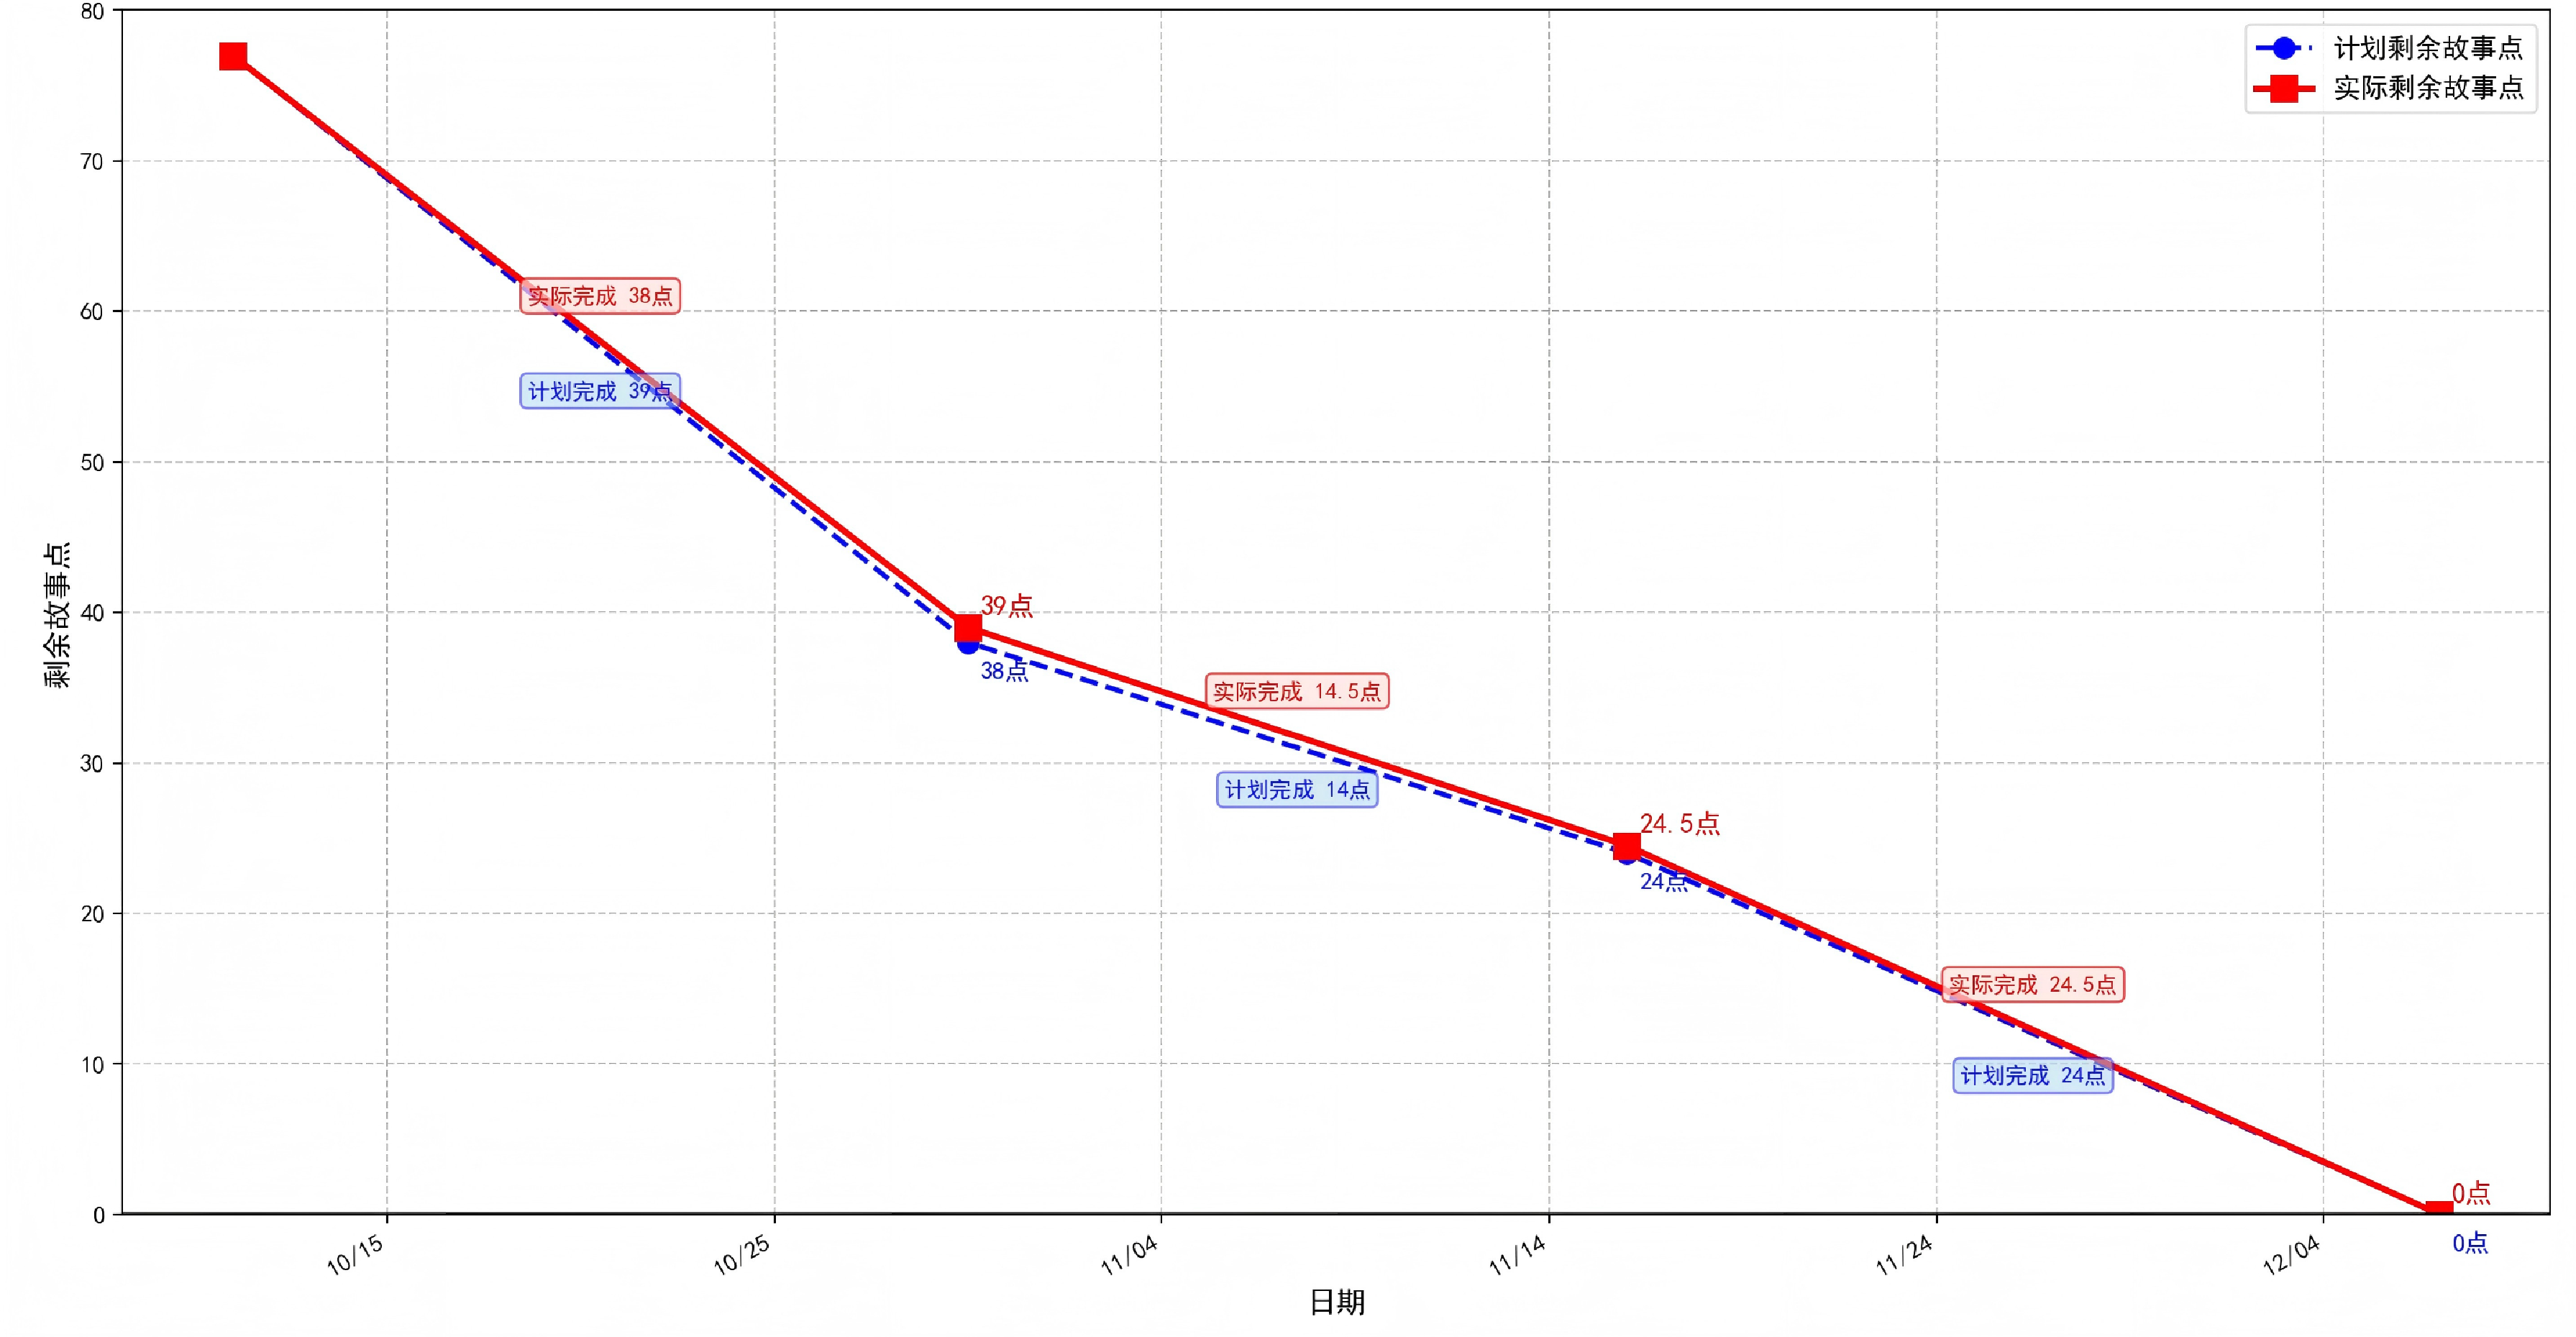
\includegraphics[width=1\textwidth]{figures/in/image5}
              \caption{整体燃尽图}
          \end{figure}

    \item \textbf{结论} \par
          \hspace{1.6em} 本项目的燃尽图清晰地展示了从启动到收尾的完整进程：虽然启动初期进度略显审慎（Sprint1剩余39点，略高于计划的38点），但团队迅速调整节奏，在后续迭代中效率稳步提升（Sprint2与Sprint3均小幅超额完成），最终确保实际燃尽线于12月7日准时归零，圆满完成了全部77个故事点的交付目标。整个过程燃尽趋势平滑健康，总计划与实际完成点数完全一致，这不仅验证了团队估算模型的可靠性，更直观体现了团队敏捷执行能力的成熟与稳定。
\end{enumerate}

\section{风险评估与规避}

\subsection{风险清单}

\begin{longtable}{>{\centering\arraybackslash}m{1cm} >{\centering\arraybackslash}m{3cm} >{\centering\arraybackslash}m{1cm} >{\centering\arraybackslash}m{1.5cm} >{\centering\arraybackslash}m{7cm}}

    \caption{风险清单} \label{tab:training}                                                                                                 \\

    \toprule
    \textbf{风险 ID} & \textbf{风险名称}        & \textbf{发生迭代} & \textbf{优先级} & \textbf{风险因素}                                                \\
    \midrule
    \endfirsthead

    \multicolumn{5}{c}{{\tablename\ \thetable{} 续表}}                                                                                    \\
    \toprule
    \textbf{风险 ID} & \textbf{风险名称}        & \textbf{发生迭代} & \textbf{优先级} & \textbf{风险因素}                                                \\
    \midrule
    \endhead

    \bottomrule
    \endfoot


    R001           & 前后端接口字段不匹配           & Sprint1       & 高            & 登录、注册、下单等接口在开发前未统一字段命名与数据结构，各自按经验实现                          \\
    R002           & 商铺 / 订单列表查询性能不达标     & Sprint1       & 中            & 商家订单列表、商铺列表初版未做分页与索引优化，高并发与大数据量下接口响应变慢                       \\
    R003           & 核心开发人员有事导致开发进度受阻     & Sprint2       & 高            & 后端曾意（负责商家接口）11.15-11.17 有其他要事                                \\
    R004           & WebSocket 断线重连与兼容性问题 & Sprint3       & 中            & 商家端订单实时推送依赖 WebSocket，网络波动或浏览器兼容性可能导致连接频繁中断                  \\
    R005           & 权限控制不严导致角色越权         & Sprint2       & 高            & 顾客、商家、管理员共用一套登录体系，如果未在路由守卫和后端同时校验角色权限，可能出现普通用户访问商家端或管理端页面的情况 \\
    R006           & 钱包与订单金额对账不一致         & Sprint3       & 高            & 钱包扣款、订单金额、退款等流程涉及多服务协作，如果缺少统一对账机制和容错设计，容易出现数据不一致             \\
    R007           & AI 客服依赖外部接口稳定性       & Sprint3       & 中            & AiChat功能依赖外部 AI 接口，如果接口限流、超时或不可用，前端体验会明显下降                   \\
    R008           & 钱包和订单相关日志过少，排障困难     & Sprint3       & 中            & 初期为了快速迭代，关键路径（支付、下单、退款）埋点不足，出问题时难以快速定位                       \\
    R009           & 表单校验不完善导致数据质量问题      & Sprint1       & 低            & 注册、商铺申请、商铺编辑等表单虽然有部分校验，但若范围、长度、必填项处理不全，可能写入脏数据               \\
    R010           & 需求变更（增加 “营业时间筛选”）    & Sprint2       & 中            & 用户反馈需增加 “按营业时间筛选商铺” 功能                                       \\
\end{longtable}


\begin{longtable}{>{\centering\arraybackslash}m{1cm} >{\centering\arraybackslash}m{1.7cm} >{\centering\arraybackslash}m{2.8cm} >{\centering\arraybackslash}m{5.2cm} >{\centering\arraybackslash}m{2.5cm}}

    \caption{风险清单（影响与应对）} \label{tab:training}                                                                                                                                                                          \\

    \toprule
    \textbf{风险 ID} & \textbf{风险名称}        & \textbf{影响}                                  & \textbf{应对措施}                                                                                     & \textbf{应对成本（工时 / 资源）}   \\
    \midrule
    \endfirsthead

    \multicolumn{5}{c}{{\tablename\ \thetable{} 续表}}                                                                                                                                                                    \\
    \toprule
    \textbf{风险 ID} & \textbf{风险名称}        & \textbf{影响}                                  & \textbf{应对措施}                                                                                     & \textbf{应对成本（工时 / 资源）}   \\
    \midrule
    \endhead

    \bottomrule
    \endfoot


    R001           & 前后端接口字段不匹配           & 导致联调阶段频繁报错，Sprint1 内用户注册 / 下单流程无法打通，影响核心功能交付 & 1）Sprint 计划会中新增“接口字段确认”环节，前后端共同评审接口文档；2）每日站会中必须汇报接口变更与联调进度；3）增加“通过 Postman / 前端集成联调用例”的检查项        & 0.5 人日（评审与联调时间增加）        \\
    R002           & 商铺 / 订单列表查询性能不达标     & 用户端加载商铺列表卡顿；商家端订单管理页面加载缓慢，影响体验与接单效率          & 1）在 Product Backlog 中新增“列表分页与索引优化”技术故事，纳入 Sprint2；2）评审会上演示接口响应时间基线；3）将性能指标写入后续迭代的 AC              & 2 人日（后端索引与分页改造 + 前端分页适配） \\
    R003           & 核心开发人员有事导致开发进度受阻     & 商家接口开发停滞，影响 Sprint2 目标                       & 1）Sprint 规划时为关键任务指定备份人员；2）请假前进行任务交接，备份人员提前熟悉代码                                                    & 2 小时（交接培训）               \\
    R004           & WebSocket 断线重连与兼容性问题 & 商家端无法及时收到新订单提醒，只能依赖手动刷新，降低接单及时性              & 1）在 Sprint3 中加入“WebSocket 健壮性优化”任务，完善断线重连与错误处理；2）每日站会跟踪线上异常日志情况；3）将“新订单实时刷新”作为订单模块 AC             & 1.5 人日（前端重连逻辑与测试）        \\
    R005           & 权限控制不严导致角色越权         & 敏感数据（商家订单、审核信息）被非授权用户查看或操作，造成数据泄露与误操作        & 1）在 Sprint2 技术任务中加入“角色权限矩阵梳理”；2）在路由守卫中校验用户角色信息；3）后端接口增加注解或拦截器强制校验角色；4）回顾会中检查是否出现越权日志              & 1.5 人日（权限方案设计 + 前后端实现）   \\
    R006           & 钱包与订单金额对账不一致         & 用户账单与订单金额对不上，引发投诉；需要人工核对，运维成本高               & 1）在 Product Backlog 中增加“账务对账工具”故事；2）在 Sprint3 中实现“订单表与钱包流水表的对账脚本”；3）每日定时任务跑对账并在异常时报警；4）回顾会上评估异常比例 & 2 人日（对账脚本与报警配置）          \\
    R007           & AI 客服依赖外部接口稳定性       & 用户在咨询问题时频繁失败或长时间无响应，对新功能好感度下降                & 1）在 Sprint3 中加入“AI 接口降级方案”任务：失败时回退到 FAQ 文本答复；2）在评审会上演示正常与降级两种路径；3）监控 AI 接口调用失败率                   & 1 人日（前端降级逻辑与简单 FAQ）      \\
    R008           & 钱包和订单相关日志过少，排障困难     & 线上问题不能快速还原，影响 MTTR（平均恢复时间），影响后续性能与安全优化       & 1）将“日志与监控完善”作为跨 Sprint 的持续改进事项；2）在 Sprint3 中为钱包 / 订单关键接口补充结构化日志；3）每日查看错误日志并在站会上同步典型问题             & 1 人日（埋点与日志规范）            \\
    R009           & 表单校验不完善导致数据质量问题      & 产生异常数据（如负数配送费、超长店铺名称），后端报错或展示异常              & 1）在 Sprint1 回顾中记录问题，并在 Sprint2 中统一梳理所有表单校验规则；2）将“前端校验 + 后端二次校验”写入开发规范；3）将关键表单校验通过作为 AC 之一         & 1 人日（规则梳理与实现）            \\
    R010           & 需求变更（增加 “营业时间筛选”）    & 打乱 Sprint2 原有计划，增加开发量                        & 1）Product Owner 评估优先级（定为 P1），纳入 Sprint3 Backlog；2）同步更新 Product Backlog，通知团队需求调整                   & 0 小时（仅调整计划）              \\
\end{longtable}


\subsection{风险跟踪与闭环}

\begin{longtable}{>{\centering\arraybackslash}m{1cm} >{\centering\arraybackslash}m{1.4cm} >{\centering\arraybackslash}m{1cm} >{\centering\arraybackslash}m{5cm} >{\centering\arraybackslash}m{4.5cm}}

    \caption{风险跟踪与闭环} \label{tab:training}                                                                                                                                                                                                                      \\

    \toprule
    \textbf{风险 ID} & \textbf{处理状态} & \textbf{处理时间} & \textbf{处理结果}                                                                                               & \textbf{后续监控措施}                                                                              \\
    \midrule
    \endfirsthead

    \multicolumn{5}{c}{{\tablename\ \thetable{} 续表}}                                                                                                                                                                                                            \\
    \toprule
    \textbf{风险 ID} & \textbf{处理状态} & \textbf{处理时间} & \textbf{处理结果}                                                                                               & \textbf{后续监控措施}                                                                              \\
    \midrule
    \endhead

    \bottomrule
    \endfoot


    R001           & 已解决           & 10 月 26 日     & 通过在 Sprint1 中补充接口字段评审会，统一了注册 / 登录 / 订单等核心接口字段，并更新接口文档；之后联调未再出现大面积字段不匹配问题。                                   & Sprint2、Sprint3 的 Sprint 计划会继续保留“接口对齐”议程；功能分支合并前必须附带接口文档变更记录。                                \\
    R002           & 处理中           & 11 月 10 日     & 已在 Sprint2 中引入订单与商铺列表分页接口，并在测试环境完成性能验证；历史接口正在逐步替换。                                                          & 每日站会跟踪分页改造任务；评审会上展示接口响应时间；计划在 11 月 17 日前完成旧接口下线。                                             \\
    R003           & 未发生           & -             & 后端人员高效处理手头事务，备份人员未启用                                                                                        & Sprint3 前确认所有成员的可参与开发时间                                                                      \\
    R004           & 未发生           & -             & 已预先在 MerchantOrders.vue中加入简单的断线重连逻辑，测试环境未发现严重问题。                                                            & 在 Sprint3 灰度发布阶段重点监控 WebSocket 错误日志和商家反馈，如出现频繁断线立即提报到 Backlog，并在下一 Sprint 优先修复。              \\
    R005           & 处理中           & 11 月 18 日     & 已根据角色矩阵梳理出顾客 / 商家 / 管理员各自可访问的页面和接口；前端路由守卫已加入基础角色判断，后端正在逐步补充接口级别的鉴权。                                         & 通过日志定期抽查敏感接口访问记录；每次安全相关回顾会议复盘是否出现越权访问；新模块上线前必须更新角色矩阵。                                        \\
    R006           & 未完成           & -             & 对账脚本与异常报警方案已在设计中，尚未落地到生产环境，仍存在潜在对账风险。                                                                       & 在下一次 Sprint 计划会中将“账务对账工具”优先级提高；上线后每日定时跑对账并在回顾会通报异常比例。                                        \\
    R007           & 已解决           & 11 月 25 日     & 已在 AI 客服前端集成降级方案，当 AI 接口超时或失败时自动切换到本地 FAQ，不再出现长时间无响应。                                                       & 监控 AI 接口超时 / 失败率；如出现异常突增，在站会上讨论是否需要调整调用频率或服务。                                                \\
    R008           & 处理中           & 11 月 22 日     & 已为关键订单与钱包接口补充基础结构化日志，但尚未统一日志规范与集中查询入口。                                                                      & 在后续迭代中推动“日志规范统一”任务；每次线上故障复盘时评估日志是否足够支撑排障，不足则补充。                                              \\
    R009           & 已解决           & 11 月 12 日     & 在 Sprint2 中统一梳理注册、商铺申请和编辑表单校验规则，前端补充长度 / 范围校验，后端增加二次校验，测试环境中已无脏数据写入。                                        & 新增表单功能时需在任务描述中附带“校验规则说明”；Code Review 清单中加入“表单校验完整性”检查项。                                      \\
    R010           & 已解决           & 11 月 5 日      & Product Owner 在评审会上确认“营业时间筛选”为 P1，但不插入当前 Sprint2；已将该需求拆分为用户故事并纳入 Sprint3 的 Product Backlog，仅调整计划，无额外开发工时投入。 & 在后续 Sprint 计划会中复核 R010 对应用户故事是否被正确排期；在每次需求评审时记录新增需求数量和对当前 Sprint 的影响，若频繁发生则在回顾会上讨论控制需求变更的机制。 \\
\end{longtable}